\chapter{Algorytmy przybliżonego zliczania}
\thispagestyle{chapterBeginStyle}
\label{rozdzial1}

W tym rozdziale  opiszemy problem zliczania oraz trzy  algorytmy przybliżonego zliczania, na których będzie się opierała dalsza cześć pracy:  \texttt{MinCount},  \texttt{Streaming MinCount} oraz \texttt{HyperLogLog}. Omówimy ich działanie, związane z nimi szkice danych, a także obciążenie i koncentrację opartych na tych szkicach estymatorów. Przedstawimy również pełny kod algorytmów. 
%%JL Następnie omówimy także naiwne metody estymacji 
%%operacji teoriomnogościowych dla tych algorytmów.


\section{Problem zliczania}
Najpierw zdefiniujmy czym jest problem zliczania, którego dotyczy nasza praca.
Zacznijmy od zdefiniowania pojęcia \textit{multizbioru}. Multizbiór $\mathfrak{M}$ definiujmy jako parę $(S, m)$, gdzie $S$ jest zbiorem nazywanym \textit{zbiorem fundamentalnym} , natomiast $m$ jest funkcją postaci $m : S \rightarrow \mathbb{N}_{\geq 1}$. Wartość $m(s)$ nazywamy mnogością elementu $s \in S$. Problem zliczania możemy zatem sformułować w taki sposób: mając multizbiór $\mathfrak{M}$, znaleźć moc $n$ zbioru fundamentalnego $S$.

W ogólnym przypadku, nie posiadając żadnych informacji na temat danych, aby znaleźć dokładne rozwiązanie tego problemu potrzebujemy liniowej pamięci $O(n)$. Zatem, próba zmniejszenia zapotrzebowania pamięci algorytmu poniżej tego poziomu musi mieć wpływ na jego dokładność i skutkuje zmniejszeniem dokładności ostatecznego wyniku. Na szczęście jeśli jesteśmy w stanie kontrolować ten błąd i jest on stosunkowo niewielki - wówczas taki algorytm jest wystarczający w większości praktycznych zastosowań i daje nam satysfakcjonunjący wynik.


\section{Algorytm MinCount}
\label{mincount}

Pierwszym algorytmem przybliżonego zliczania, którym się zajmiemy jest \texttt{MinCount} znany również pod innymi nazwami, np.  \texttt{K-th Minimum Value} (KMV) \cite{kmv}. Algorytm ten opiera się na statystykach pozycyjnych.

\subsubsection{Statystyki pozycyjne}

Rozważmy  zmienne losowe $X_1, X_2, \dots, X_n$. Statystykami pozycyjnymi będziemy nazywać zmienne losowe  $X_{(1)}, X_{(2)}, \dots, X_{(n)}$ powstałe przez posortowanie realizacji zmiennych $X_1, X_2, \dots, X_n$ rosnąco.  Zmienną $X_{(k)}$ nazywamy k-tą statystyką pozycyjną. W szczególności $X_{(1)} = \min\{X_1, X_2, \dots, X_n \}$. W dalszej części pracy będziemy zakładać, że
zmienne $X_1, X_2, \dots X_n$ są niezależne i każda  ma rozkład jednostajny na odcinku (0,1).

Przyjmijmy, że istnieje funkcja haszująca 
\begin{equation}
    h \colon \mathfrak{M} \rightarrow (0, 1)
\end{equation}
taka, że jeśli $\mathfrak{M}$ posiada $n$ unikalnych elementów $a_1, a_2, \dots a_n$ to przyjmując, że
 $U_i = h(a_i)$ otrzymamy ciąg niezależnych zmiennych losowych o rozkładzie jednostajnym $U_1, U_2, \dots U_n \sim U(0,1)$. Zauważmy również, że jeśli element $a_i$ pojawia się w  $\mathfrak{M}$ wielokrotnie, to zawsze będzie zhaszowany do tej samej wartości.
 
Rozważmy statystyki pozycyjne  $U_{(1)}, U_{(2)}, \dots, U_{(n)}$ powstałe przez posortowanie realizacji  $U_1, U_2, \dots U_n$. O zmiennej losowej $U_{(k)}$ wiemy, że pochodzi z rozkładu $Beta(\alpha, \beta)$, gdzie $\alpha = k, \beta = n + 1 - k$ i jest zdefiniowana przez następującą funkcję rozkładu prawdopodobieństwa \cite{mincount}:
\begin{equation}
    f(x; \alpha, \beta) = \frac{x^{\alpha-1}{(1-x)}^{\beta-1}}{B(\alpha, \beta)},
\end{equation} 
gdzie $$B(\alpha, \beta) = \frac{\Gamma(\alpha)\Gamma(\beta)}{\Gamma(\alpha + \beta)}$$ przy czym funkcja $\Gamma(z)$ jest nazywana \textit{gammą Eulera} i definiuje się ją jako: $$\Gamma(z) = \int_0^\infty t^{z-1}e^{-t} dt$$
Łatwo pokazać, że wartość oczekiwana zmiennej losowej $X$ pochodzącej z rozkładu $Beta(\alpha, \beta)$ jest funkcją stosunku parametrów $\alpha$ i $\beta$:
\begin{equation}
    E[X] = \int_0^1 xf(x; \alpha, \beta) dx = \int_0^1 x\frac{x^{\alpha-1}{(1-x)}^{\beta-1}}{B(\alpha, \beta)} dx = \frac{\alpha}{\alpha + \beta} .
\end{equation}
Stąd mamy
\begin{equation}
\label{OS-expexcation}
E[\frac{1}{U_{(k)}}] = \int_0^1 \frac{1}{x}f(x; k, n + 1 - k) dx = \frac{n}{k-1}.
\end{equation}
 
 \subsubsection*{Estymator liczności}
 
 Wykorzystując formułę (\ref{OS-expexcation}) oraz metodę momentów, możemy  zdefiniować estymator liczności $\hat{n}$ naszego zbioru wejściowego $a_1, a_2, \dots a_n$ jako:
\begin{equation}
    \hat{n} = \frac{k - 1}{U_{(k)}}
    \label{mincount_est}
\end{equation}
Pokażemy teraz, że estymator $\hat{n}$ jest estymatorem nieobciążonym, gdy $k \geq 2$:
\begin{flalign}
    E[\hat{n}] = \int_0^1 \frac{k - 1}{x}f(x; k, n+1-k) dx \\
    = (k - 1)\int_0^1 \frac{1}{x}f(x; k, n+1-k) dx \\
    = (k-1)\frac{n}{k-1} = n
\end{flalign}
Podobnie, możemy policzyć wariancję estymatora \cite{mincount}, gdy $k \geq 3$:
\begin{flalign}
    Var[\hat{n}] =  E[{\hat{n}}^2] - {E[\hat{n}]}^2 \\
    = \frac{k-1}{k-2}n(n-1) - n^2 \\
    = \frac{(k-1)n(n-1) - n^{2}(k-2)}{k-2}  \\
    = \frac{n(n - k + 1)}{k - 2}
\end{flalign}
Przy czym, dla $n \rightarrow \infty$ możemy zapisać:
\begin{equation}
	Var[\hat{n}] \approx \frac{n^2}{k-2}
	\label{mincount_var}
\end{equation}

\subsubsection{Szkic danych}
Zdefiniujemy szkic danych algorytmu \texttt{MinCount}. Szkic $S$ określamy jako parę $(H, {\tau})$, gdzie $H$ to zbiór $k$ najmniejszych (i unikalnych) haszy spośród wszystkich wartości $h(\mathfrak{M})$. Natomiast ${\tau}$ to wartość k-tej statystyki pozycyjnej, czyli największa wartość w zbiorze haszy $H$.
%\AW{Zmienilem oznaczenie zbioru haszy z S na H, żeby nie myliło się ze szkicem - czyli szkic $S = (H, \tau)$}
\subsubsection{Algorytm \texttt{MinCount}}

Algorytm \texttt{MinCount} opisany w poniższym pseudokodzie działa w następujący sposób.
Początkowo w szkicu mamy $H = \emptyset$ i $\tau = 0$.
Jeśli w chwili pojawienia się nowego elementu wejściowego $x$
 ze strumienia $\mathfrak{M}$ rozmiar $|H|< k$ wówczas dodajemy $x$ do $H$ i ustalamy $\tau$ jako największą wartość z $H$.
 Jeśli rozmiar $|H|\geq k$ to porównujemy hasz $h(x)$ z aktualną wartością  ${\tau}$ szkicu. Jeżeli jest mniejsza, to dodajemy $h(x)$ do zbioru $H$, usuwamy z niego dotychczasowe ${\tau}$ i ustalamy nowe.

W oparciu o szkic $(H, {\tau})$ jesteśmy w stanie w dowolnym momencie wyliczyć wartość estymatora liczności $$\hat{n} := \frac{k - 1}{{\tau}}.$$

\begin{algorithm}
    \begin{algorithmic}
    \State $k$ -  liczba przechowywanych haszy 
    \State $H  $ - zbiór przechowywanych haszy
    \State $\tau  $ - największy przechowywany hasz 
    \State $h  $ - funkcja haszująca elementy $\mathfrak{M}$ w odcinek $(0, 1)$
    \newline
    \Function{Add}{$x \in \mathfrak{M}$}
        \State $e \gets h(x)$
        \If {$e \notin S$}
            \If {$H.size < k$}
                \State $H.add(e)$
                \State $\tau \gets max\{H\}$
            \ElsIf {$e < \tau$}
                \State $H.remove(\tau)$
                \State $H.add(e)$
                \State $\tau \gets max\{H\}$
            \EndIf
        \EndIf
    \EndFunction
    \newline
    \Function{Estimate}{} 
        \If {$H.size < k$} 
            \State \Return $H.size$
        
        \Else 
            \State \Return $(k - 1) / \tau$
        \EndIf
    \EndFunction
    
    \end{algorithmic}
    \caption{Algorytm \texttt{MinCount}}
\end{algorithm}

%\AW{Dla zwyklego MinCounta tez wrzucic histogram? jesli tak to jak go skomentowac - ze niespecjalnie podchodzi pod rozklad normalny? czy ze troche podchodzi ale nie tak dobrze jak streamingMC?}
%\JL{Prosze sprobowac tak zrobic, zobaczymy jak to bedzie wygladac.}

Na wykresie \ref{fig:mincount_hist} zamieszczamy histogram prezentujący rozkład błędu względnego tego algorytmu dla ok. $10^5$ eksperymentów, z parametrem $k=100$. Jak możemy zauważyć, rozkład wartości błędu na histogramie nie jest tak podobny do krzywej rozkładu normalnego, jak w przypadku algorytmów, które omówimy w następnej kolejności: \texttt{Streaming MinCount} oraz \texttt{HyperLogLog}. Fakt ten jest dosyć istotny i uzasadnia wybór \texttt{Streaming MinCount} jako algorytmu, którym docelowo będziemy posługiwać się w rozdziale \ref{weighted_method}.
%\AW{Moze cos takiego? Nie umiem tego zbyt ladnie sformulowac..}
%\JL{Jest OK}
\begin{figure}[h!]
	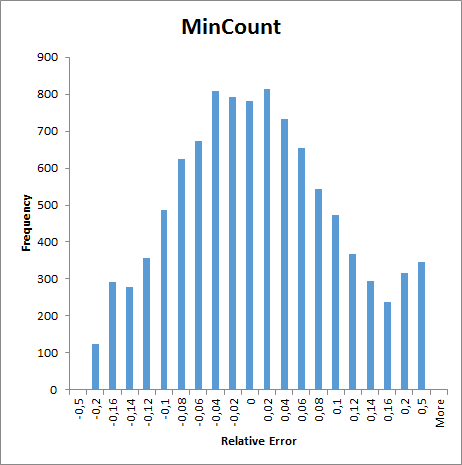
\includegraphics[width=0.5\textwidth]{MinCountErrHist.png}
	\centering
	\caption{Rozkład błędu względnego dla algorytmu \texttt{MinCount} przy $10^5$ eksperymentach}
	\label{fig:mincount_hist}
\end{figure}
\newpage

\section{Algorytm Streaming MinCount}
\label{smincount}

Jednym z mniej znanych algorytmów opartych na statystykach pozycyjnych, który będziemy rozważać w dalszej części pracy jest algorytm \texttt{Streaming MinCount} \cite{streamed}. Algorytm ten różni się od klasycznego \texttt{MinCounta} sposobem estymacji liczności. Wykorzystuje on taki sam szkic, ale wykonuje tzw. \textit{estymację kroczącą}. Tzn. wykorzystuje do estymacji również informacje o zmianach w szkicu, a nie tylko końcową postać szkicu:
\begin{equation}
    \hat{n} = \sum_{t \in T} \frac{Z_t}{\tau_{t}}
    \label{streaming_est}
\end{equation}
gdzie $\tau_{t}$ to wartość największego spośród $k$ przechowywanych haszy po przetworzeniu $t$ elementów $\mathfrak{M}$, a $Z_t$ jest zmienną binarną przyjmującą wartość $1$ jeśli szkic zmienił się w momencie $t$ lub $0$ w p.p. Jak widać ten estymator operuje na przestrzeni czasu $t$, tzn. każdy kolejny napotkany element ze strumienia wejściowego inkrementuje $t$. Dzięki takiemu podejściu, estymator zmienia wartość tylko wtedy, gdy hasz nowo napotkanego elementu modyfikuje szkic. Wykorzystanie dodatkowych informacji o zmianach w szkicu powoduję zmniejszenie wariancji estymatora o połowę względem klasycznego algorytmu \texttt{MinCount} \cite{ting}. Analiza tego estymatora wraz ze szczegółowym opisem i dowodem własności znajduje się w pracy \cite{streamed}. Poniżej przedstawiamy 
pseudokod dla algorytmu \texttt{Streaming MinCount}:
\newline
\begin{algorithm}
    \begin{algorithmic}
    \State $k $ - liczba przechowywanych haszy 
    \State $H  $ - zbiór przechowywanych haszy
    \State $\tau  $ - największy przechowywany hasz 
    \State $h  $ - funkcja haszująca elementy $\mathfrak{M}$ w odcinek $(0, 1)$
    \State $\hat{n} \gets 0$  - estymator liczności
    \newline
    \Function{Add}{$x \in \mathfrak{M}$}
        \State $e \gets h(x)$
        \If {$e \notin H$}
            \If {$H.size < k$}
                \State $H.add(e)$
                \State $\tau \gets max\{H\}$
                \State $\hat{n} \gets \hat{n} + (1/\tau)$
            \ElsIf {$e < \tau$}
                \State $H.remove(\tau)$
                \State $H.add(e)$
                \State $\tau \gets max\{H\}$
                \State $\hat{n} \gets \hat{n} + (1/\tau)$
            \EndIf
        \EndIf
    \EndFunction
    \newline
    \Function{Estimate}{} 
        \State \Return $round(\hat{n})$
    \EndFunction
    
    \end{algorithmic}
    \caption{Algorytm \texttt{Streaming MinCount}}
\end{algorithm}

Na wykresie \ref{fig:str_mincount_hist} zamieszczamy również histogram prezentujący rozkład błędu względnego tego algorytmu dla ok. $10^5$ eksperymentów, z parametrem $k=100$. Jak możemy wnioskować z wykresu, dla dużej liczby eksperymentów błąd względny zaczna mieć rozkład bardzo zbliżony do rozkładu normalnego. Ta obserwacja przyda nam się w dalszej części pracy do uzasadnienia pewnych założeń dotyczących nowych metod estymacji.

\begin{figure}[h!]
	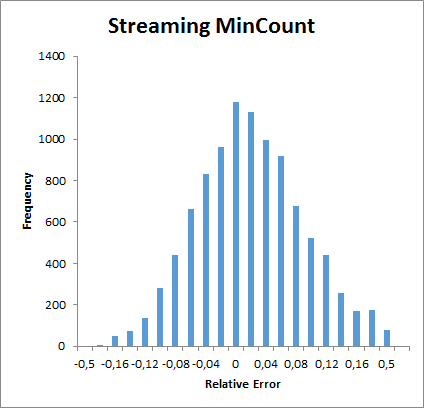
\includegraphics[width=0.5\textwidth]{StreamingMinCountErrHist.png}
	\centering
	\caption{Rozkład błędu względnego dla algorytmu \texttt{StreamingMinCount} przy $10^5$ eksperymentach}
	\label{fig:str_mincount_hist}
\end{figure}

\section{Algorytm HyperLogLog}
\label{hll}

Trzecim algorytmem przybliżonego zliczania, który omówimy w tej pracy jest \texttt{HyperLogLog} zaprezentowany w pracy \cite{hll}. Podobnie jak w algorytmie \texttt{MinCount}  haszuje on elementy wejściowego  multizbioru $\mathfrak{M}$ w odcinek $(0,1)$. Jednak tym razem hasze są traktowane nie jak liczby w zapisie binarnym, a jak ciągi złożone z zer i jedynek. Algorytm na bieżąco śledzi maksymalną liczbę zer wiodących wśród wszystkich haszy. Idea algorytmu jest następująca: przy założeniu, że na każdej pozycji zero i jedynka pojawia się z jednakowym prawdopodobieństwem,  hasze które zawierają więcej zer wiodących są rzadziej spotykane. Wskazują zatem na większą liczność zbioru wejściowego. Innymi słowy, jeśli ciąg bitów postaci $0^{q-1}1$ pojawi się na początku hasza, wówczas przy założeniu, że funkcja $h$ zwraca wartości zgodnie z rozkładem jednostajnym, możemy estymować liczbę różnych elementów multizbioru wejściowego na $2^{q}$.

Takie podejście oparte na pojedynczym eksperymencie posiada jednak dużą wariancję. Aby zmniejszyć warinację stosuję się technikę znaną jako stochastyczne uśrednianie (ang. \textit{stochastic averaging}). Strumień wejściowy $\mathfrak{M}$ dzielony jest na $m$ mniejszych podstrumieni $\mathfrak{M}_i$ podobnych rozmiarów. O tym, do którego podstrumienia należeć będzie dany element decyduje $p$ początkowych bitów z jego hasza, gdzie $m = 2^p$. Następnie te $p$ początkowych bitów jest usuwane z $h(x)$ i dla  każdego $x\in \mathfrak{M}_i$ wyznaczana jest pozycja $q$ pierwszej jedynki z tak powstałego $h(x)$. Największe ze znalezionych pozycji $q$ w każdym podstrumieniu przetrzymywane są w tablicy rejestrów $M$, tzn. w $M[i]$ jest największą  wartość $q$
dla  podstrumienia $\mathfrak{M}_i$:
\begin{equation}
    M[i] = \max_{x \in \mathfrak{M}_i} Q(x)
\end{equation}
gdzie $Q(x)$ jest funkcją zwracającą  pozycję pierwszej jedynki w haszu elementu $x$.
 Korzystając z tych rejestrów algorytm wylicza estymację liczby różnych elementów $\hat{n}$
 jako średnią harmoniczną, skorygowaną o współczynnik ${\alpha}_{m}$ usuwający obciążenie estymatora:
\begin{equation}
    \hat{n} = {\alpha}_m{m}^{2}(\sum_{i=1}^{m} 2^{-M[i]}),
\end{equation}
gdzie
\begin{equation}
    {\alpha}_{m} = (m \int_{0}^{\infty} ({\log}_2(\frac{2 + u}{1 + u}))^m du)^{-1}.
\end{equation}
Można pokazać, że dla  $n \rightarrow \infty$, wartość oczekiwana dla powyższego estymatora ma postać (zobacz \cite{hll}):
\begin{equation}
    E[\hat{n}] = n(1 + {\delta}_1(n) + o(1)),
\end{equation}
gdzie $|{\delta}_1(n)| < 5 \times 10^{-5}$ dla $m \geq 16$, wariancja natomiast wynosi:
\begin{equation}
    Var[\hat{n}] = (n(\frac{{b}_m}{\sqrt{m}} + {\delta}_2(n) + o(1)))^2,
    \label{hll_var}
\end{equation}
 gdzie $|{\delta}_2(n)| < 5 \times 10^{-4}$ dla $m \geq 16$, a stała ${b}_m$ jest ograniczona i wynosi odpowiednio dla: 
 \begin{itemize}
 	\item ${b}_{16} \approx 1.106$, 
 	\item ${b}_{32} \approx 1.070$, 
 	\item ${b}_{64} \approx 1.054$, 
 	\item ${b}_{128} \approx 1.046$, 
 	\item ${b}_{\infty} = \sqrt{3\log{2} - 1} \approx 1.03896$. 
 \end{itemize}
 Funkcje ${\delta}_1(n)$ oraz ${\delta}_1(n)$ są funkcjami oscylującymi o małej amplitudzie i mogą zostać bezpiecznie pominięte w zastosowaniach praktycznych.

Wyniki eksperymentalne pokazały jednak, że przedstawiona powyżej wersja algorytmu nie sprawdza się dla wszystkich zakresów wartości $n$, dlatego twórcy wprowadzili do algorytmu pewne korekcje:
\begin{enumerate}
    \item Poprawka dla małych liczności - symulacje przeprowadzone przez autorów algorytmu wykazały, że jeśli liczba rożnych elementów $n \le \frac{5}{2}m$, 
    to pojawiają się istotne zaburzenia. Dlatego dla tego zakresu liczności $n$ autorzy sugerują użycie  algorytmu \texttt{Linear Counting} \cite{linear} jako estymatora:
    \begin{equation}
    \hat{n} = {m}log(\frac{m}{V})
    \label{LC}
    \end{equation}
    gdzie $m = 2^p$, a $V$ to liczba rejestrów równych $0$.
    
    \item Poprawka dla dużych liczności - gdy wartość $n$ zbliża się do $2^{32} \approx 4 \times 10^9$, kolizje haszy stają się coraz bardziej prawdopodobne (jeśli używamy standardowo 32-bitowej funkcji haszującej). Aby temu zapobiec zastosowano również stosowną korekcję. Jeśli wartość estymatora $\hat{n}$ jest większa niż $\frac{2^{32}}{30}$ wówczas jego ostateczna wartość zostaje zastąpiona przez:
    \begin{equation}
	    \hat{n} = {-2}^{32}log(1 - \frac{\hat{n}}{2^{32}})
    \end{equation}
    Wzór ten wynika z podstawienia do wzoru (\ref{LC}) wartości $m = 2^{32}$ oraz $V = 2^{32} - \hat{n}$ oraz odwrócenia zawartości logarytmu.
\end{enumerate}
Szczegółowo algorytm oraz powyższe korekcje zostały opisane przez twórców w \cite{hll} wraz ze wszystkimi własnościami.

\subsubsection{Szkic danych}
\label{HLL_sketch}
Parametrami wejściowymi dla szkicu są $p$ oraz $q$, gdzie $p + q$ określa liczbę używanych bitów funkcji haszującej. Parametr $p$ wyznacza liczbę rejestrów, a więc tym samym kontroluje błąd względny, natomiast $q$ wyznacza maksymalny zakres wartości dla rejestrów. Warto zauważyć, że jeśli liczność zbioru zbliża się do $2^{p+q}$ kolizje haszy stają się coraz częstsze i błąd znacznie wzrasta. 
Szkicem danych algorytmu \texttt{HyperLogLog} jest kolekcja rejestrów $M[i]$ przechowujących największą napotkaną pozycję pierwszej jedynki w haszach podstrumienia $\mathfrak{M}_i$, gdzie $i = 1 ... m$, $m = 2^p$ wyznacza liczbę rejestrów. Szkic ten możemy w naturalny sposób wykorzystać do wyznaczenia estymatora \texttt{Linear Counting} potrzebnego do zastosowania korekcji $1.$ Zauważmy, że szkic, dla którego parametr $q = 0$ jest równoważny tablicy bitowej używanej w algorytmie \texttt{Linear Counting}. Wystarczy zatem, że zliczymy ile spośród rejestrów jest równych $0$ (oznaczmy liczbę pustych rejestrów przez $V$) ignorując wartości pozostałych rejestrów i zastosujemy wzór (\ref{LC}).

 Poniżej przedstawiamy pseudokod algorytmu \texttt{HyperLogLog} z zastosowaniem opisanych wcześniej korekcji:
\newline
\begin{algorithm}
    \begin{algorithmic}
    \State $p $ - parametr wejściowy sterujący liczbą rejestrów
    \State $q $ - parametr wejściowy wyznaczający zakres wartości rejestrów
    \State $m \gets 2^p$ - liczba rejestrów
    \State ${\alpha}_m $ - współczynnik korygujący obciążenie
    \State $Q(s) $ -  funkcja zwracając pozycję pierwszej jedynki w ciągu bitów $s$ 
    \State $h(x)  $  - $(p + q)$-bitowa funkcja haszująca $\mathfrak{M}$ w $(0, 1)$
    \State $M $  - kolekcja $m$ rejestrów 
    \newline
    \For {$i = 1 .. m$}
        \State $M[i] \gets 0$
    \EndFor
    \newline
    \Function{Add}{$x \in \mathfrak{M}$}
        \State $e \gets h(x)$
        \State $idx \gets 1 + {{\langle}e_1, e_2, ..., e_b{\rangle}}_2$
        \State $v \gets e_{b+1}, e_{b+2}, ...$
        \State $M[idx] \gets max\{M[idx], Q(v)\}$
    \EndFunction
    \newline
    \Function{Estimate}{} 
        \State $\hat{n} \gets {\alpha}_{m}{m}^2(\sum_{j=0}^{m} 2^{(-M[j])})^{-1}$
        \If {$\hat{n} \leq \frac{5}{2}m$}
            \State $V \gets $ liczba rejestrów $M[i]$ równych $0$
            \If {$V > 0$}
                \State $\hat{n} \gets {m}\log(\frac{m}{V})$
            \EndIf
        \ElsIf {$\hat{n} > \frac{1}{30}2^{32}$}
            \State $\hat{n} \gets -2^{32}\log(1 - \frac{\hat{n}}{2^{32}})$
        \EndIf
        \State \Return $\hat{n}$
    \EndFunction
    
    \end{algorithmic}
    \caption{Algorytm \texttt{HyperLogLog}}
\end{algorithm}

%\JL{Najlepiej wygenerować samemu, ale można napisać że jest też w pracy z HLL i najlepiej to zdanie, że to wynika z usredniania- tzn. liczenia sredniej harmonicznej i CTG}
%\AW{Dodalem histogram + komentarz}
%\JL{OK}
Na wykresie \ref{fig:hll_hist} prezentujemy histogram z rozkładem błędu względnego dla algorytmu \texttt{HyperLogLog} dla ok. $10^5$ przeprowadzonych eksperymentów, przy $m=2^{10}$. Jak sugerują autorzy \cite{hll}, oczekiwany rozkład powinien być zbliżony o rozkładu normalnego, ze względu na efekt \textit{uśredniania} oraz w oparciu o \textit{Centralne Twierdzenie Graniczne}, co potwierdzają przeprowadzone przez nas (oraz przez autorów) empiryczne testy.

\begin{figure}[h!]
	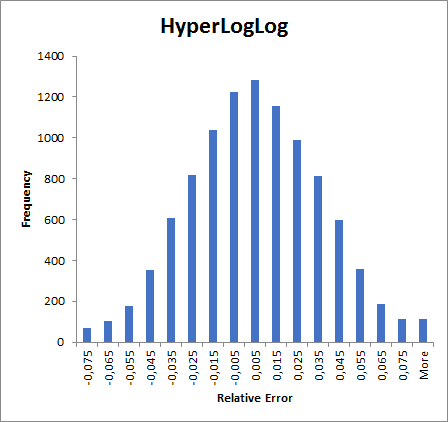
\includegraphics[width=0.5\textwidth]{HLLErrHist.png}
	\centering
	\caption{Rozkład błędu względnego dla algorytmu \texttt{HyperLogLog} przy $10^5$ eksperymentach}
	\label{fig:hll_hist}
\end{figure}